% Copyright 2021 Fausto Spoto
%
% Licensed under the Apache License, Version 2.0 (the "License");
% you may not use this file except in compliance with the License.
% You may obtain a copy of the License at
%
%    http://www.apache.org/licenses/LICENSE-2.0
%
% Unless required by applicable law or agreed to in writing, software
% distributed under the License is distributed on an "AS IS" BASIS,
% WITHOUT WARRANTIES OR CONDITIONS OF ANY KIND, either express or implied.
% See the License for the specific language governing permissions and
% limitations under the License.

\documentclass[11pt]{beamer}  %% versione proiettore
%%\documentclass[11pt,handout]{beamer} %% versione stampa
\usepackage{lucidiJb-2ed}
\usepackage{mathtools}
\usepackage{relsize}
\usepackage[normalem]{ulem}

\mode<article>
{
  \usepackage{fullpage}
  \usepackage{hyperref}
}

\mode<presentation>
{
  \setbeamertemplate{background canvas}[vertical shading][bottom=red!10,top=blue!10]
  \usetheme{Course}
  \usefonttheme[onlysmall]{structurebold}
}

\subtitle{Blockchain Course}
\title{Hotmoka}
\institute{Universit\`a di Verona, Italy}
\date{March 2021}

\setbeamercovered{invisible}

\def\codesize{\smaller}
\def\<#1>{\codeid{#1}}
\newcommand{\codeid}[1]{\ifmmode{\mbox{\codesize\ttfamily{#1}}}\else{\codesize\ttfamily #1}\fi}

\begin{document}

\begin{frame}
  \titlepage
\end{frame}

\begin{frame}
  \frametitle{Hotmoka}

  \begin{greenbox}{\url{https://github.com/Hotmoka/hotmoka}}
    An open-source implementation of a network of nodes:
    \begin{itemize}
    \item nodes of a blockchain
    \item IoT devices
    \item computers in the cloud
    \end{itemize}
  \end{greenbox}

  \bigskip

  \begin{greenbox}{Requests are OO-based}
    \begin{itemize}
    \item create an object
    \item call a method of an object
    \item methods are implemented in a subset of Java
    \end{itemize}
  \end{greenbox}

\end{frame}

\begin{frame}\frametitle{Documentation}

  \begin{greenbox}{}
    There is an online tutorial on Hotmoka and Takamaka
    in the \<README.md> of the main repository of Hotmoka:

    \url{https://github.com/Hotmoka/hotmoka}
  \end{greenbox}

  \bigskip

  \begin{greenbox}{}
    Its examples of Takamaka projects are available here:

    \url{https://github.com/Hotmoka/hotmoka_tutorial}
  \end{greenbox}

\end{frame}

\begin{frame}\frametitle{The API of a Hotmoka node}

  \begin{itemize}
  \item \<[add|post]JarStore(request):TransactionReference>
  \item \<[add|post]ConstructorCall(request):StorageReference>
  \item \<[add|post|run]InstanceMethodCall(request):StorageValue>
  \item \<[add|post|run]StaticMethodCall(request):StorageValue>
  \item \<subscribeToEvents(key):Subscription>
  \item \<getState(StorageReference):State>
  \end{itemize}

  \bigskip

  \begin{greenbox}{}
    \<add> calls are synchronous (wait for the result)

    \smallskip
    \<post> calls are asynchronous (yield a future)

    \smallskip
    \<run> calls are synchronous and only for read-only methods
  \end{greenbox}

\end{frame}

\begin{frame}\frametitle{Nodes can be Tendermint applications}

  \begin{center}
    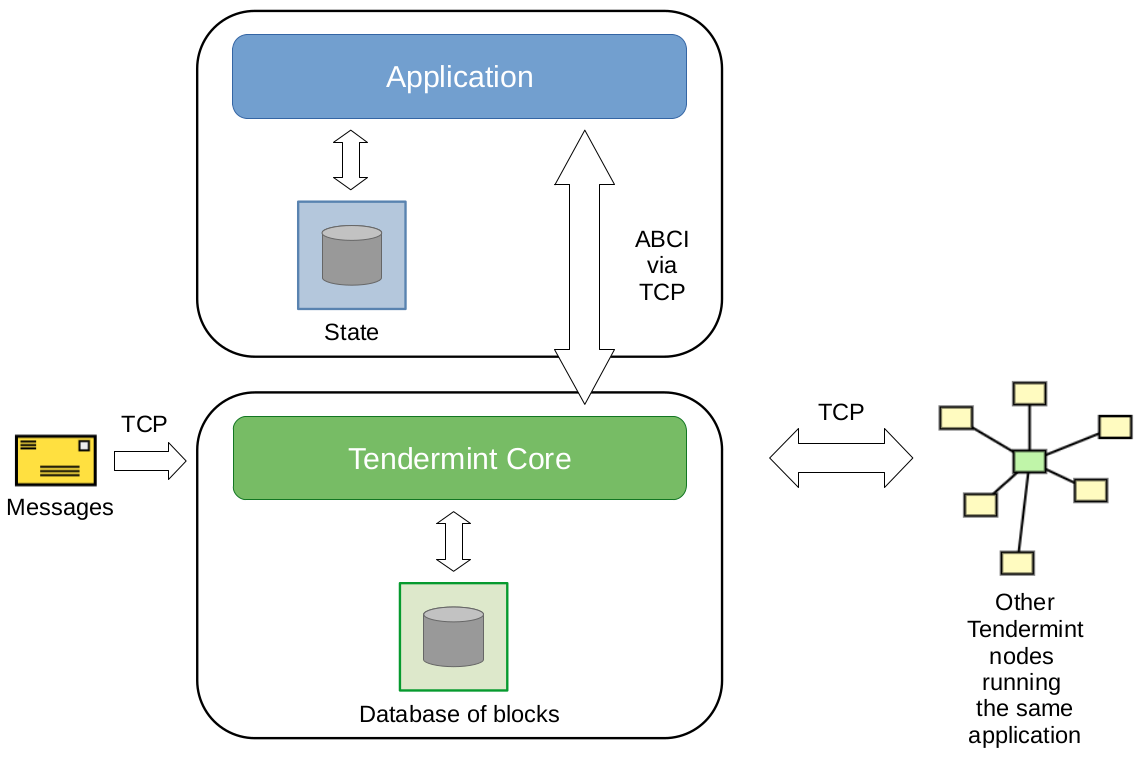
\includegraphics[width=\textwidth,clip=false]{pictures/tendermint-databases.png}
  \end{center}
    
\end{frame}

\begin{frame}\frametitle{An OO state (hash is sha256)}

  \begin{center}
    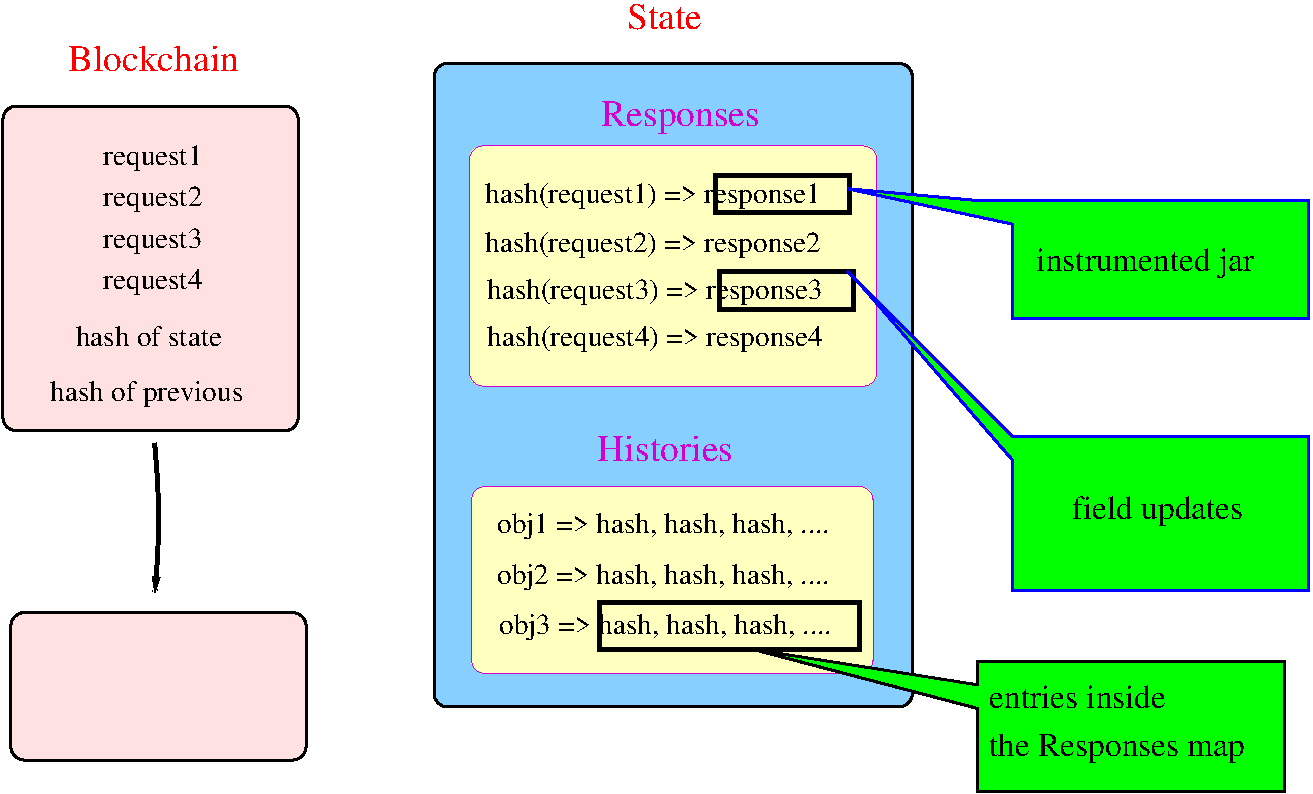
\includegraphics[width=\textwidth,clip=false]{pictures/hotmoka-structure.pdf}
  \end{center}

\end{frame}

\begin{frame}\frametitle{The API of the state}
  
    \begin{enumerate}
    \item get jar at \<hash>: access the Responses map and find the jar
    \item get object at \<obj>: access the Histories at \<obj>: for each \<hash>
      there, access the Responses map at \<hash>, project the updates on \<obj>
      and reconstruct the state of \<obj>
    \item put request/response in state: expand Responses with hash(request)$\Rightarrow$response
      \begin{itemize}
      \item[] if the response contains updates, add hash(request) to the histories of
        the updated objects
      \end{itemize}
    \item \<h=get\_hash()>: compute the hash of the hash of the Merkle-Patricia trie for
      Responses and of that for Histories
    \item \sout{\<checkout(h)>} $\Rightarrow$ unused data from points above are garbage-collected
    \end{enumerate}

\end{frame}

\begin{frame}[fragile]\frametitle{Start experimenting with Hotmoka}

  \begin{enumerate}
  \item ensure to have Java version $\ge$ 11 installed

  \item ensure to have git and Maven installed

  \item download Hotmoka

    {\color{blue}\<git clone git@github.com:Hotmoka/hotmoka.git>}

  \item let Maven compile and install it in your local Maven repository

    {\color{blue}\<mvn clean install -DskipTests>}

  \end{enumerate}

\end{frame}

% How I started the node:
%java --module-path modules/explicit:modules/automatic --class-path "modules/unnamed/*" --module io.hotmoka.tools/io.hotmoka.tools.CLI init-tendermint 1000000000000000000000000000000000000 --open-unsigned-faucet

\begin{frame}[fragile]\frametitle{Info about a Hotmoka node}

  A Hotmoka node over Tendermint has been published on AWS for the duration of this course

  \bigskip

  \begin{greenbox}{Run this inside the Hotmoka repository (on a single line!)}
    {\small\begin{semiverbatim}
java {\color{red}--module-path modules/explicit:modules/automatic
     --class-path "modules/unnamed/*"}
     {\color{blue}--module io.hotmoka.tools/io.hotmoka.tools.CLI} info
     --url ec2-54-194-239-91.eu-west-1.compute.amazonaws.com:8080
    \end{semiverbatim}}
  \end{greenbox}

  \medskip

  \begin{greenbox}{You can define an alias to simplify the command (single line!)}
    {\small\begin{semiverbatim}
alias CLI='java --module-path modules/explicit:modules/automatic
                --class-path "modules/unnamed/*"
                --module io.hotmoka.tools/io.hotmoka.tools.CLI'
    \end{semiverbatim}}
  \end{greenbox}

  \medskip

  \begin{greenbox}{Use the alias instead}
{\small\<CLI info --url ec2-54-194-239-91.eu-west-1.compute.amazonaws.com:8080>}
  \end{greenbox}

\end{frame}

\begin{frame}[fragile]\frametitle{\<CLI info --url ec2....>}

{\tiny\begin{semiverbatim}
 {\color{red}takamakaCode:} 02dfd29348abaa44f720525179fa170f26063c973fd40c3ff368a9402551882c
 {\color{red}manifest:} 42a8a11aee0405aee5775514b3b0456c7740bbb015b4b87df4776e6e4add7668#0
   chainId: {\color{violet}chain-ASdWiN}
   maxErrorLength: 300
   maxDependencies: 20
   maxCumulativeSizeOfDependencies: 10000000
   allowsSelfCharged: false
   {\color{violet}allowsUnsignedFaucet: true}
   skipsVerification: false
   signature: ed25519
   {\color{red}gamete:} 4f7d7ca1fbea152d8f323c21e1abcfa1d979c7c4ea667d8457381a26b08a2d71#0
     balance: 999999999999999999999999999999992180
     redBalance: 0
     {\color{violet}maxFaucet: 1000000}
     maxRedFaucet: 0
   {\color{red}gasStation:} 42a8a11aee0405aee5775514b3b0456c7740bbb015b4b87df4776e6e4add7668#10
     {\color{violet}gasPrice: 1}
     maxGasPerTransaction: 1000000000
     ignoresGasPrice: false
     targetGasAtReward: 1000000
     inflation: 10000 (ie. 0.10%)
     oblivion: 250000 (ie. 25.00%)
   {\color{red}validators:} 42a8a11aee0405aee5775514b3b0456c7740bbb015b4b87df4776e6e4add7668#2
     {\color{violet}number of validators: 1}
     validator #0: 42a8a11aee0405aee5775514b3b0456c7740bbb015b4b87df4776e6e4add7668#1
       id: C220489CDBAE0FAFF8F8286A9C541FD55BA2CE7C 
       power: 1
     ticketForNewPoll: 100
     number of polls: 0
   {\color{red}versions:} 42a8a11aee0405aee5775514b3b0456c7740bbb015b4b87df4776e6e4add7668#f
     verificationVersion: 0
  \end{semiverbatim}}

\end{frame}

\begin{frame}\frametitle{The minimal content of a Hotmoka node's state}

  \begin{center}
    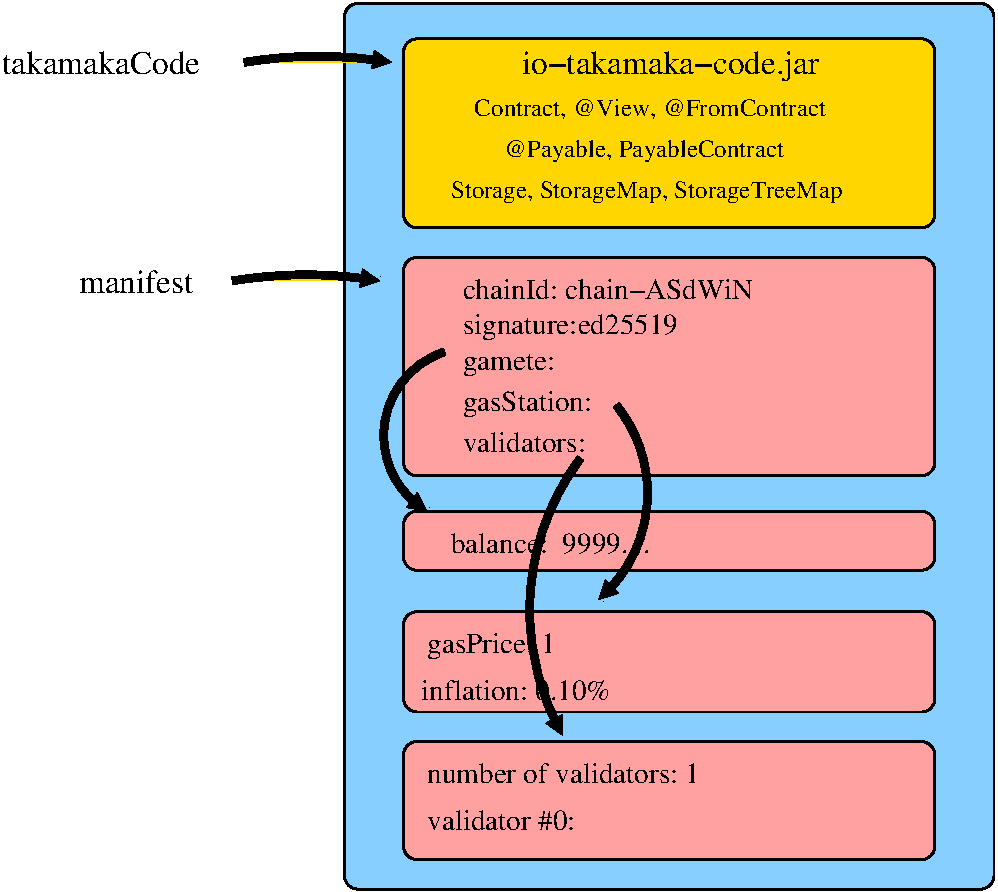
\includegraphics[scale=0.5,clip=false]{pictures/state1.pdf}
  \end{center}
  
\end{frame}

\begin{frame}[fragile]\frametitle{The state contains actual Java objects}

  {\scriptsize
    \texttt{manifest:} $\underbrace{{\color{red}\mathtt{42a8a11aee0405aee5775514b3b0456c7740bbb015b4b87df4776e6e4add7668\#0}}}_{\text{machine-independent memory address of an object}}$
  }

  \bigskip

  \begin{greenbox}{{\scriptsize\<CLI state 42a8a11aee0405aee5775514b3b0456c7740bbb015b4b87df4776e6e4add7668\#0 --url ec2...>}}
    {\tiny\begin{semiverbatim}
class {\color{violet}io.takamaka.code.governance.Manifest} (from jar installed at 02dfd29348abaa44f7205251...)
  allowsSelfCharged:boolean = false
  allowsUnsignedFaucet:boolean = true
  chainId:java.lang.String = "chain-ASdWiN"
  gamete:io.takamaka.code.lang.Account = {\color{red}4f7d7ca1fbea152d8f323c21e1abcfa1d979c7c4ea667d8457381a26b08a2d71#0}
  gasStation:io.takamaka.code.governance.GasStation = {\color{red}42a8a11aee0405aee5775514b3b0456c7740bbb015b4b8...}
  maxCumulativeSizeOfDependencies:long = 10000000
  maxDependencies:int = 20
  maxErrorLength:int = 300
  signature:java.lang.String = "ed25519"
  skipsVerification:boolean = false
  validators:io.takamaka.code.governance.Validators = {\color{red}42a8a11aee0405aee5775514b3b0456c7740bbb015b4b8...}
  versions:io.takamaka.code.governance.Versions = {\color{red}42a8a11aee0405aee5775514b3b0456c7740bbb015b4b87df4...}
^ balance:java.math.BigInteger = 0 {\color{violet}(inherited from io.takamaka.code.lang.Contract)}
^ balanceRed:java.math.BigInteger = 0 {\color{violet}(inherited from io.takamaka.code.lang.Contract)}
^ nonce:java.math.BigInteger = 227 {\color{violet}(inherited from io.takamaka.code.lang.ExternallyOwnedAccount)}
^ publicKey:java.lang.String = "" {\color{violet}(inherited from io.takamaka.code.lang.ExternallyOwnedAccount)}
    \end{semiverbatim}}
  \end{greenbox}

\end{frame}

\begin{frame}[fragile]\frametitle{Creation of a new account}

  Let us create a new account with 500000 units of coin:

  \smallskip

  \begin{greenbox}{{\small\<CLI create-account 500000 --payer faucet --url ec2...>}}
    {\tiny\begin{semiverbatim}
Free account creation will succeed only if the gamete of the node supports an open unsigned faucet
{\color{armygreen}total gas consumed: 3791}
{\color{darkred}  for CPU: 620
  for RAM: 1574
  for storage: 1597
  for penalty: 0}
A new account 06aa6a1afabc82c7161ffcdc2391a2136101aaeb94f64edd53a1d0d1436d610e\#0 has been created
{\color{blue}The keys of the account have been saved
  into the file 06aa6a1afabc82c7161ffcdc2391a2136101aaeb94f64edd53a1d0d1436d610e\#0.keys}
    \end{semiverbatim}}
  \end{greenbox}

  \bigskip

  \begin{redbox}{Who paid for that?}
    Gas and coins have been paid by the gamete, then provides an unsigned \emph{faucet}.
    This is a testnet. A real network has no open unsigned faucet
    and one must specify the address of the payer account then
    (with \<--payer>)
  \end{redbox}

\end{frame}

\begin{frame}[fragile]\frametitle{Let us have a look at our first account}

    \begin{greenbox}{{\scriptsize\<CLI state 06aa6a1afabc82c7161ffcdc2391a2136101aaeb94f64edd53a1d0d1436d610e\#0 --url ec2...>}}
    {\tiny\begin{semiverbatim}
class {\color{violet}io.takamaka.code.lang.ExternallyOwnedAccount} (from jar installed at 02dfd29348abaa...)
  nonce:java.math.BigInteger = 0
  publicKey:java.lang.String = "MCowBQYDK2VwAyEAk45GxqvRFg88bKZqkqDGxQBHdvvZF+b9YSkl8xs28Ao="
^ balance:java.math.BigInteger = 500000 (inherited from io.takamaka.code.lang.Contract)
^ balanceRed:java.math.BigInteger = 0 (inherited from io.takamaka.code.lang.Contract)
    \end{semiverbatim}}
  \end{greenbox}

  \bigskip

  \begin{itemize}
  \item the nonce starts from 0
  \item the initial balance is actually 500000
  \item the public key a Base64-encoded ed25519 key
  \item the public key is stored in the object: no need to send it again at every future
    method call (like Ethereum does)
  \end{itemize}

\end{frame}

\begin{frame}\frametitle{A new object in state}

  \begin{center}
    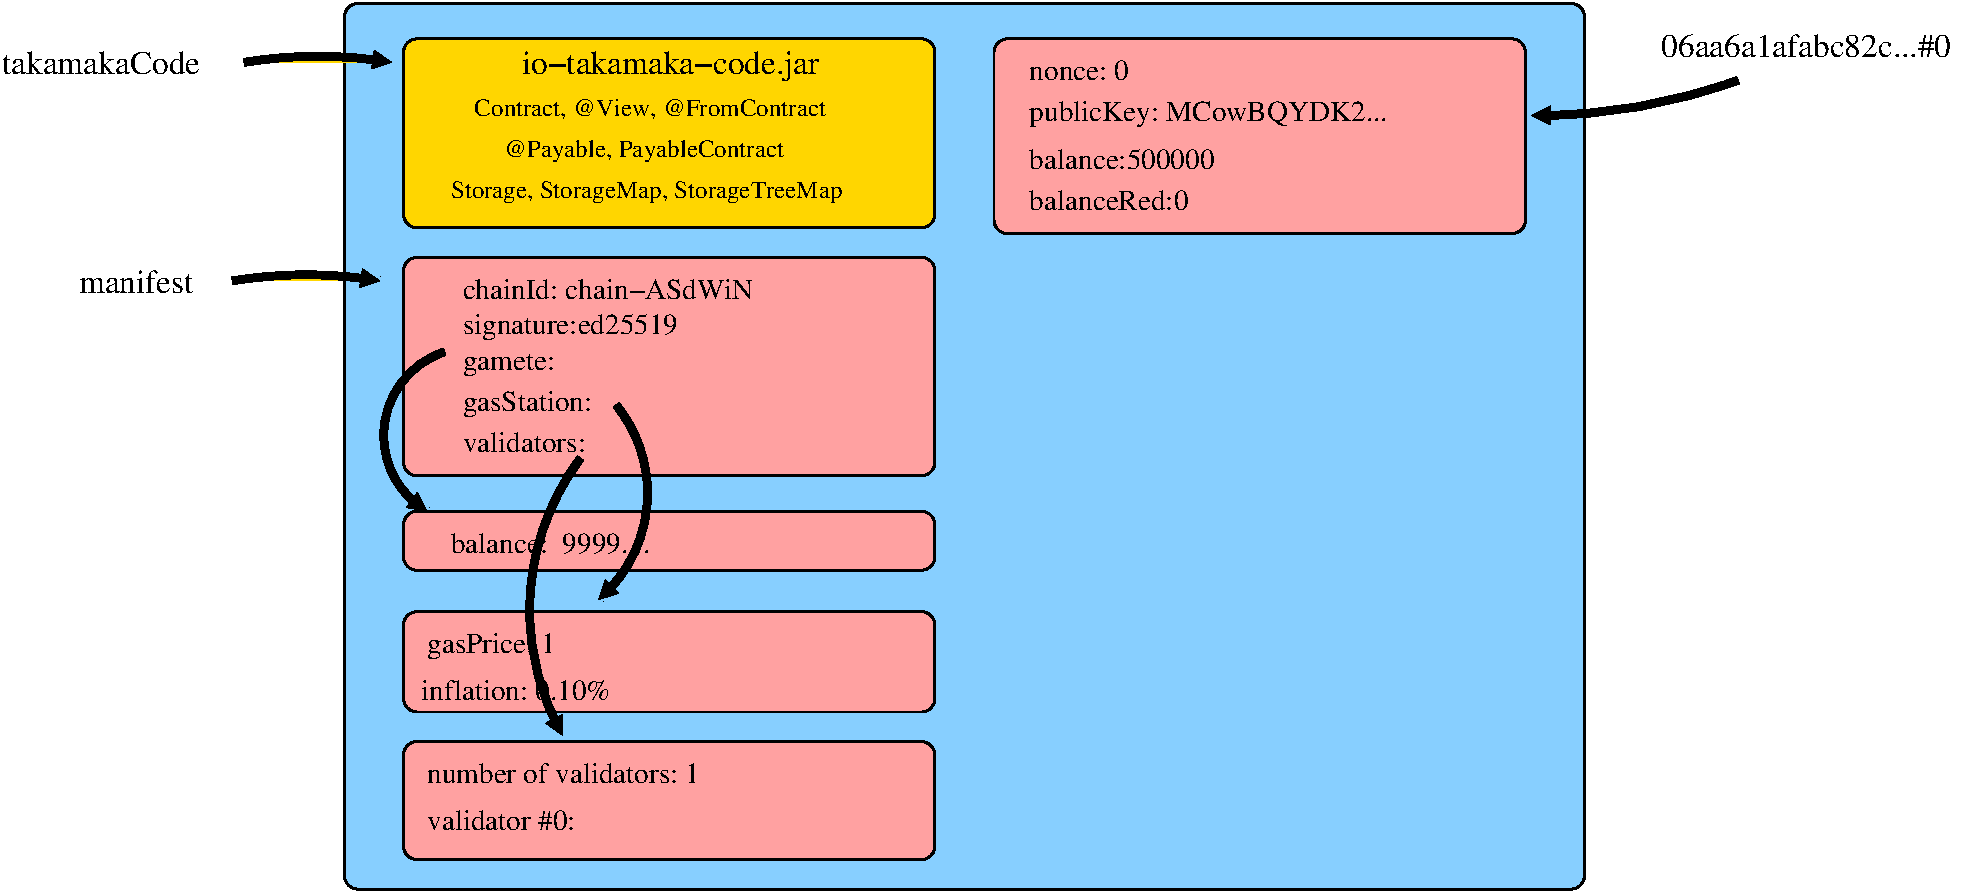
\includegraphics[scale=0.37,clip=false]{pictures/state2.pdf}
  \end{center}
  
\end{frame}

\begin{frame}[fragile]\frametitle{Let us have a look at the API of our first account}

    \begin{greenbox}{{\scriptsize\<CLI state 06aa6a1afabc82c7161ffcdc2391a2136101aaeb94f64edd53a1d0d1436d610e\#0 {\color{orange}--api} --url ec2...>}}
    {\tiny\begin{semiverbatim}
class {\color{violet}io.takamaka.code.lang.ExternallyOwnedAccount} (from jar installed at 02dfd29348abaa...)
  nonce:java.math.BigInteger = 0
  publicKey:java.lang.String = "MCowBQYDK2VwAyEAk45GxqvRFg88bKZqkqDGxQBHdvvZF+b9YSkl8xs28Ao="
^ balance:java.math.BigInteger = 500000 (inherited from io.takamaka.code.lang.Contract)
^ balanceRed:java.math.BigInteger = 0 (inherited from io.takamaka.code.lang.Contract)

  {\color{red}@Payable @FromContract} public ExternallyOwnedAccount(java.math.BigInteger,java.lang.String)
  {\color{red}@Payable @FromContract} public ExternallyOwnedAccount(long,java.lang.String)
  {\color{red}@Payable @FromContract} public ExternallyOwnedAccount(int,java.lang.String)
  public ExternallyOwnedAccount(java.lang.String)

  {\color{red}@View} public final java.math.BigInteger nonce()
  {\color{red}@View} public final java.lang.String publicKey()
  {\color{red}@View} public java.lang.String toString()
^ {\color{red}@View} public final java.math.BigInteger balance() (inherited from io.takamaka.code.lang.Contract)
^ {\color{red}@View} public final java.math.BigInteger balanceGreen() (inherited from io.takamaka.code.lang.Contract)
^ {\color{red}@View} public final java.math.BigInteger balanceRed() (inherited from io.takamaka.code.lang.Contract)
^ public final int compareByStorageReference(io.takamaka.code.lang.Storage)
    (inherited from io.takamaka.code.lang.Storage)
^ public boolean equals(java.lang.Object) (inherited from java.lang.Object)
^ public final native java.lang.Class getClass() (inherited from java.lang.Object)
^ {\color{red}@View} public final java.lang.String getClassName() (inherited from io.takamaka.code.lang.Storage)
^ public native int hashCode() (inherited from java.lang.Object)
^ {\sout{public final native void notify() (inherited from java.lang.Object)}} {\color{red}X}
^ {\sout{public final native void notifyAll() (inherited from java.lang.Object)}} {\color{red}X}
^ {\color{red}@Payable @FromContract} public final void receive(int)
    (inherited from io.takamaka.code.lang.PayableContract)
^ {\color{red}@Payable @FromContract} public final void receive(java.math.BigInteger)
    (inherited from io.takamaka.code.lang.PayableContract)
  ...
    \end{semiverbatim}}
  \end{greenbox}

\end{frame}

\begin{frame}[fragile]\frametitle{Let us call \<toString()> on our first account}

\begin{tt}
CLI call <payer> <receiver> <methodName> [<args>...]
\end{tt}

\bigskip

We will use our account as payer and as receiver at the same time:

\bigskip

\begin{greenbox}{{\small\<CLI call 06aa6a1afabc82c7161ffcdc2391a2136101aaeb94f64edd53a1d0d1436d610e\#0 06aa6a1afabc82c7161ffcdc2391a2136101aaeb94f64edd53a1d0d1436d610e\#0 toString --url ec2...>}}
    {\begin{semiverbatim}
{\color{blue}an externally owned account}
calls to @View methods consume no gas 
    \end{semiverbatim}}
  \end{greenbox}

\bigskip

\begin{center}
  \<toString()> in class \<ExternallyOwnedAccount> is annotated as \<@View>
\end{center}

\end{frame}

\begin{frame}\frametitle{The execution of a method (or constructor)}

  \begin{greenbox}{The request specifies}
    \begin{itemize}
    \item payer object, receiver object and actual arguments (\emph{input})
    \item classpath, signature of the method
    \item nonce, chain id, gas price, gas limit
    \item signature of the request
    \end{itemize}
  \end{greenbox}

  \bigskip

  \begin{greenbox}{The computation of the response (ie, the execution of the request)}
    \begin{enumerate}
    \item find the jar(s) in state for the classpath
    \item reconstruct, from the state, RAM objects for \emph{input}
    \item execute the method on a normal Java Virtual Machine (in RAM)
    \item at the end, identify updates to fields of objects reachable from \emph{input}
      or return value
    \item pack those updates into a response (RAM objects destroyed now)
    \item put request/response in state, expanding histories
    \end{enumerate}
  \end{greenbox}

\end{frame}

\begin{frame}[fragile]\frametitle{How can Hotmoka identify updates to fields of objects?}

  \begin{greenbox}{The original code}
    \begin{semiverbatim}
      public class C \{
        public {\color{blue}int i;}
        public void foo() \{
          {\color{blue}i} = 42;
        \}
      \}
    \end{semiverbatim}
  \end{greenbox}

  \begin{center}
    No way to know if \<i> changed its value during the execution of \<foo()>
  \end{center}

\end{frame}

\begin{frame}[fragile]\frametitle{How can Hotmoka identify updates to fields of objects?}

  \begin{greenbox}{The instrumented code}
    \begin{semiverbatim}
      public class C {\color{red}extends Storage} \{
        public {\color{blue}int i, old\_i;} // aliased at method start
        public void foo() \{
          {\color{blue}i} = 42;
        \}
      \}
    \end{semiverbatim}
  \end{greenbox}

  \begin{center}
    \<i> changed its value during the execution of \<foo()> iff at the end \<i>$\not=$\<old\_i>
  \end{center}

\end{frame}

\begin{frame}[fragile]\frametitle{How can Hotmoka enforce gas limits?}

  \begin{greenbox}{The original code}
    \begin{semiverbatim}
      public class C \{
        public void foo() \{
          while (...) \{
            ...
          \}
        \}
      \}
    \end{semiverbatim}
  \end{greenbox}

  \begin{center}
    This loop might run for very long or even forever
  \end{center}

\end{frame}

\begin{frame}[fragile]\frametitle{How can Hotmoka enforce gas limits?}

  \begin{greenbox}{The instrumented code}
    \begin{semiverbatim}
      {\color{blue}static long counter;}
      public class C \{
        public void foo() \{
          while (...) \{
            {\color{blue}if (counter++ >= gaslimit)
              throw new OutOfGasError();}
            ...
          \}
        \}
      \}
    \end{semiverbatim}
  \end{greenbox}

  \begin{center}
    Actual gas costs are more fine-grained
  \end{center}

\end{frame}

\begin{frame}\frametitle{Verification and instrumentation of jars in state}

  Each jar that gets installed in a Hotmoka node undergoes two processes:

  \begin{enumerate}
  \item Verification: absence of frequent errors
    \begin{itemize}
    \item objects stored in state extend \<Storage>
    \item non-deterministic or non-terminating library code is not used
    \item no synchronization
    \item no native code
    \item no \emph{dangerous} bytecodes
    \item no finalizers
    \item no static fields (mostly)
    \item code annotations are used correctly
    \item \ldots
    \end{itemize}
  \item Instrumentation
    \begin{itemize}
    \item fields of \<Storage> classes get duplicated
    \item gas metering is weaved into the code
    \item code annotations get implemented \emph{by magic}
    \item \ldots
    \end{itemize}
  \end{enumerate}

\end{frame}

\begin{frame}\frametitle{The Takamaka programming language}

  Takamaka is the subset of Java that passes the verification
  of a Hotmoka node. It uses code annotations to implement contract-based aspects:

  \begin{itemize}
  \item {\color{blue}\<@FromContract>} annotates something that can only be called by a contract,
    not by any other code; hence, it has a {\color{blue}\<caller()>}
  \item {\color{blue}\<@Payable>} annotates something whose execution requires to pay some
    cryptocurrency units
  \item {\color{blue}\<@View>} annotates something whose execution can be run for free,
    without paying for its gas: it must not generate any update at its end
    (\emph{pure} code)
  \end{itemize}

  \bigskip
  Takamaka comes equipped with a {\color{blue}support library}
  (\<io-takamaka-code>) that defines such annotations and
  other typical classes that are useful
  for programming smart contracts

\end{frame}

\begin{frame}[fragile]\frametitle{A first example of Takamaka code}

  \begin{enumerate}
  \item create a new Java Maven project (skip archetype selection)
  \item edit the Maven configuration file \<pom.xml> as follows:
\vspace*{-1ex}{\tiny\begin{semiverbatim}
{\color{blue}{
<project ...>
  <modelVersion>4.0.0</modelVersion>

  {\color{armygreen}<groupId>io.hotmoka</groupId>
  <artifactId>ponzi</artifactId>
  <version>0.0.1</version>}

  {\color{violet}{<properties>
    <project.build.sourceEncoding>UTF-8</project.build.sourceEncoding>
    <maven.compiler.source>11</maven.compiler.source>
    <maven.compiler.target>11</maven.compiler.target>
    <failOnMissingWebXml>false</failOnMissingWebXml>
  </properties>}}

  {\color{red}{<dependencies> <dependency>
      <groupId>io.hotmoka</groupId>
      <artifactId>io-takamaka-code</artifactId>
      <version>1.0.0</version>
  </dependency> </dependencies>}}

  {\color{violet}{<build> <plugins> <plugin>
        <groupId>org.apache.maven.plugins</groupId>
        <artifactId>maven-compiler-plugin</artifactId>
        <version>3.8.1</version>
        <configuration> <release>11</release> </configuration>
  </plugin> </plugins> </build>}}

</project>
}}\end{semiverbatim}}
  \end{enumerate}

\end{frame}

\begin{frame}[fragile]\frametitle{A first example of Takamaka code}

  \begin{enumerate}
    \setcounter{enumi}{2}
  \item create a source package \<io.takamaka.ponzi> inside \<src/main/java>
  \item create a \<module-info.java> in the \<src/main/java> directory:
    \vspace*{-3ex}\begin{semiverbatim}
{\color{blue}{
module ponzi \{
  requires io.takamaka.code;
\}
}}\end{semiverbatim}
  \end{enumerate}

\end{frame}

\begin{frame}[fragile]\frametitle{A first example of Takamaka code}

  \begin{enumerate}
    \setcounter{enumi}{4}
      \item add the following class in package \<io.takamaka.ponzi>
\vspace*{-1ex}{\tiny\begin{semiverbatim}
{\color{darkblue}{
package io.takamaka.ponzi;

import static io.takamaka.code.lang.Takamaka.require;
import java.math.BigInteger;
import io.takamaka.code.lang.Contract;
import io.takamaka.code.lang.FromContract;
import io.takamaka.code.lang.Payable;
import io.takamaka.code.lang.PayableContract;
import io.takamaka.code.lang.View;

public class SimplePonzi {\color{red}extends Contract} \{
  private final BigInteger _10 = BigInteger.valueOf(10L), _11 = BigInteger.valueOf(11L);
  private {\color{armygreen}PayableContract} currentInvestor;
  private BigInteger currentInvestment = BigInteger.ZERO;

  public {\color{violet}@Payable} {\color{armygreen}@FromContract(PayableContract.class)} void invest({\color{violet}BigInteger amount}) \{
    BigInteger minimum = currentInvestment.multiply(_11).divide(_10);
    require(amount.compareTo(minimum) >= 0, () -> "you must invest at least " + minimum);

    if (currentInvestor != null)
      currentInvestor.{\color{armygreen}receive(amount)};

    currentInvestor = {\color{armygreen}(PayableContract) caller()};
    currentInvestment = amount;
  \}

  public {\color{red}@View} BigInteger getCurrentInvestment() \{
    return currentInvestment;
  \}
\}
}}\end{semiverbatim}}
  \end{enumerate}

\end{frame}

\begin{frame}[fragile]\frametitle{A first example of Takamaka code}

  \begin{enumerate}
    \setcounter{enumi}{5}
  \item compile and package everything with Maven:

    {\color{blue}\<mvn package>}

  \item the compiled \<ponzi-0.0.1.jar> will appear inside the
    \<target> directory of your project, ready to be installed in a
    Hotmoka node

  \item install \<ponzi-0.0.1.jar> in our AWS Hotmoka node (\begin{tt}CLI install <payer> <jar>\end{tt})
  \end{enumerate}

  \medskip

  \begin{greenbox}{{\small\<CLI install 06aa6a1afabc82c7161ffcdc2391a2136101aaeb94f64edd53a1d0d1436d610e\#0 .../target/ponzi-0.0.1.jar --url ec2...>}}
    {\scriptsize\begin{semiverbatim}
Do you really want to spend up to 23732 gas units to install the jar [Y/N] Y
.../target/ponzi-0.0.1.jar has been installed at
  {\color{red}39f999a63555542eaf5040388d61c20193dee4fb035847a40608c494bf069765}
{\color{armygreen}total gas consumed: 3583}
{\color{darkred}  for CPU: 252
  for RAM: 1260
  for storage: 2071
  for penalty: 0}
    \end{semiverbatim}}
  \end{greenbox}

\end{frame}

\begin{frame}\frametitle{A new jar in state}

  \begin{center}
    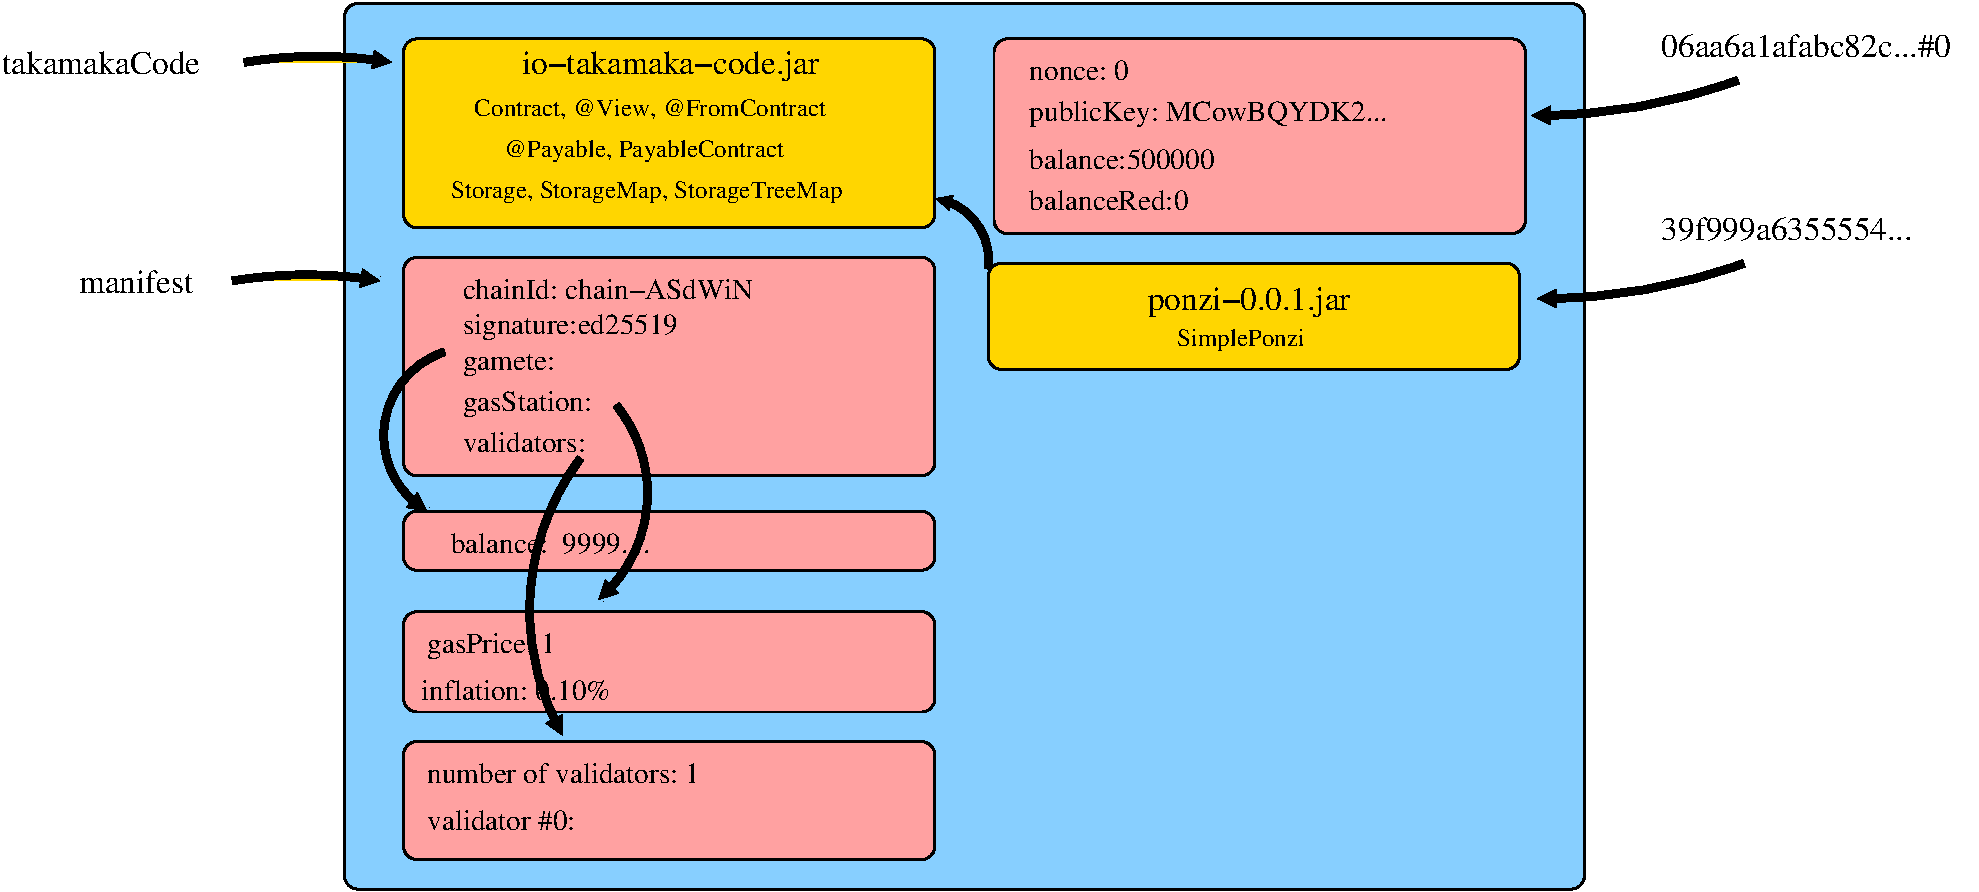
\includegraphics[scale=0.37,clip=false]{pictures/state3.pdf}
  \end{center}
  
\end{frame}

\begin{frame}[fragile]\frametitle{Creation of a new object in state}

\begin{tt}
CLI create <payer> <className> [<args>...]
\end{tt}

\bigskip

We use our account as payer and specify where \<SimplePonzi> is defined
(the \alert{classpath}):

\bigskip

\begin{greenbox}{{\small\<CLI create 06aa6a1afabc82c7161ffcdc2391a2136101aaeb94f64edd53a1d0d1436d610e\#0 io.takamaka.ponzi.SimplePonzi
      \newline --classpath 39f999a63555542eaf5040388d61c20193dee4fb035847a40608c494bf069765
      --url ec2...>}}
    {\tiny\begin{semiverbatim}
do you really want to spend up to 10000 gas units to call {\color{red}public SimplePonzi()} ? [Y/N] Y
the new object has been allocated at 754371b03ef2c413f546e1c3667adf86d545a3587e60f75d2c496863ef442f5c\#0
{\color{armygreen}total gas consumed: 3107}
{\color{darkred}  for CPU: 299
  for RAM: 1209
  for storage: 1599
  for penalty: 0}
    \end{semiverbatim}}
  \end{greenbox}

\end{frame}

\begin{frame}\frametitle{A new \<SimplePonzi> in state}

  \begin{center}
    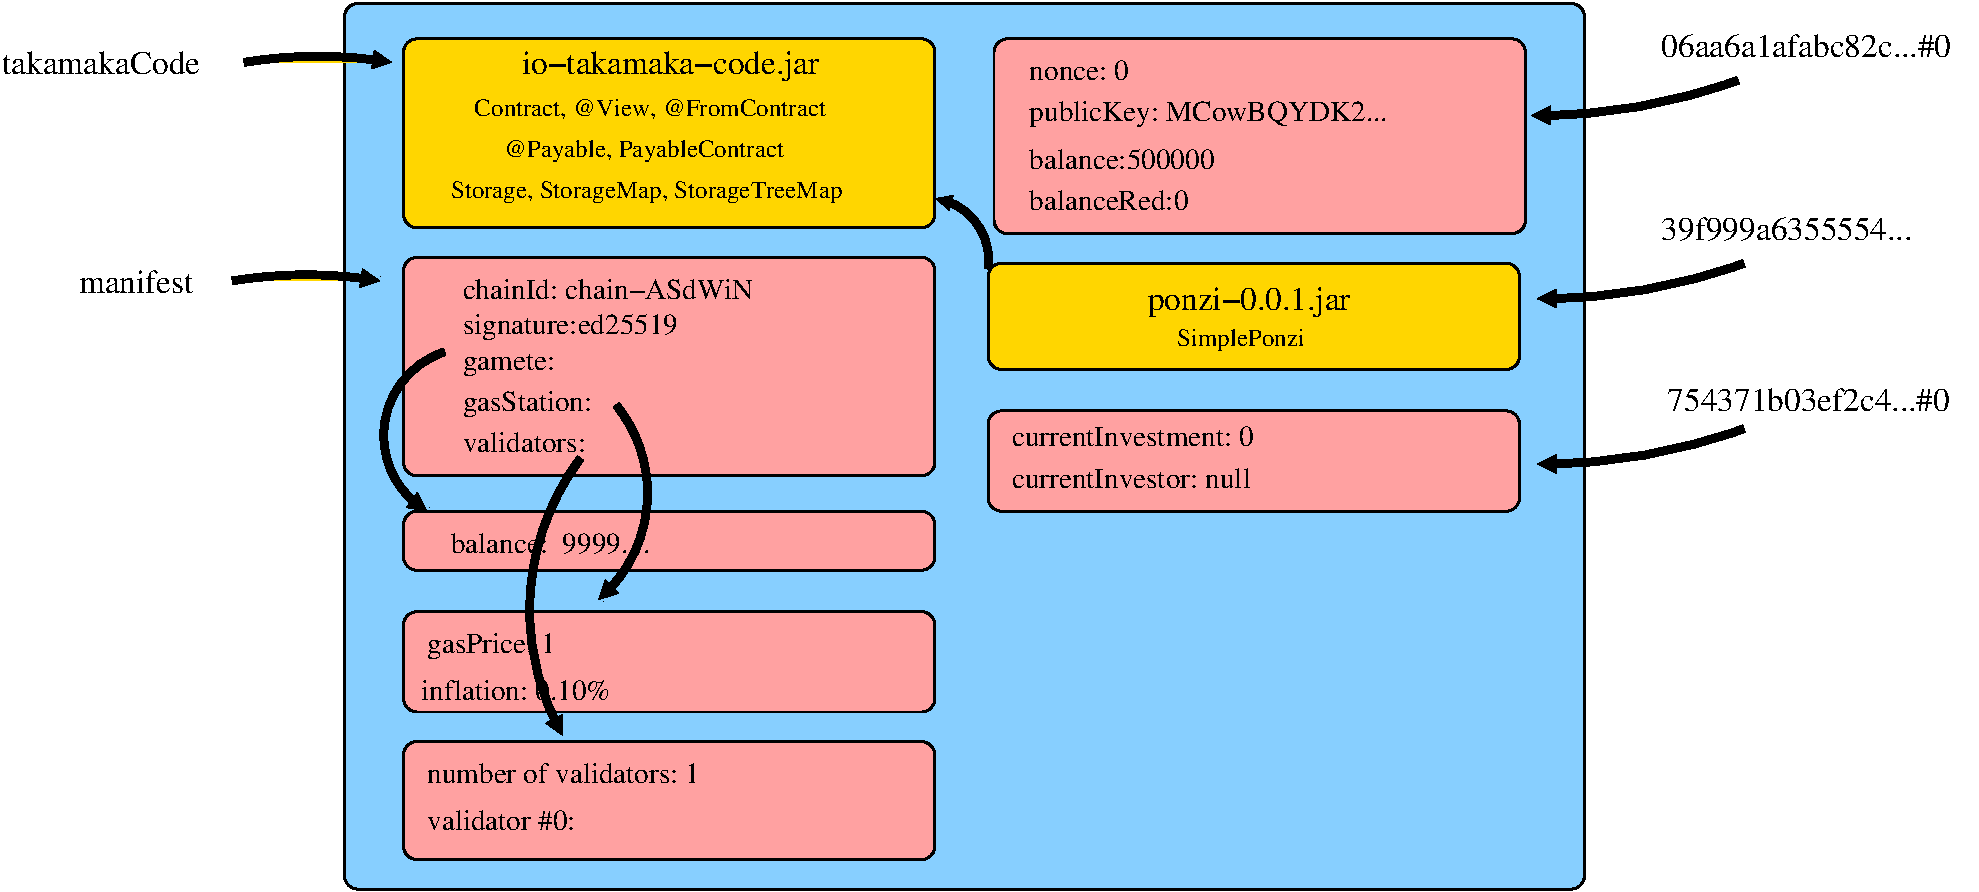
\includegraphics[scale=0.37,clip=false]{pictures/state4.pdf}
  \end{center}
  
\end{frame}

\begin{frame}[fragile]\frametitle{Call the \<invest> method of our contract}

\begin{tt}
CLI call <payer> <receiver> <methodName> [<args>...]
\end{tt}

\medskip

We use our account as payer:

\medskip

\begin{greenbox}{{\small\<CLI call 06aa6a1afabc82c7161ffcdc2391a2136101aaeb94f64edd53a1d0d1436d610e\#0 754371b03ef2c413f546e1c3667adf86d545a3587e60f75d2c496863ef442f5c\#0 invest 40000
      --url ec2...>}}
    {\tiny\begin{semiverbatim}
do you really want to spend up to 10000 gas units to call
  {\color{red}@Payable @FromContract(PayableContract.class) public void invest(java.math.BigInteger)} ? [Y/N] Y
{\color{armygreen}total gas consumed: 2112}
{\color{darkred}  for CPU: 421
  for RAM: 1349
  for storage: 342
  for penalty: 0}
    \end{semiverbatim}}
  \end{greenbox}

\end{frame}

\begin{frame}[fragile]\frametitle{Call the \<invest> method of our contract, again}

\begin{tt}
CLI call <payer> <receiver> <methodName> [<args>...]
\end{tt}

\medskip

We use our account as payer:

\medskip

\begin{greenbox}{{\small\<CLI call 06aa6a1afabc82c7161ffcdc2391a2136101aaeb94f64edd53a1d0d1436d610e\#0 754371b03ef2c413f546e1c3667adf86d545a3587e60f75d2c496863ef442f5c\#0 invest 40000
      --url ec2...>}}
    {\tiny\begin{semiverbatim}
do you really want to spend up to 10000 gas units to call
  {\color{red}@Payable @FromContract(PayableContract.class) public void invest(java.math.BigInteger)} ? [Y/N] Y
{\color{armygreen}total gas consumed: 10000}
{\color{darkred}  for CPU: 465
  for RAM: 1449
  for storage: 342
  for penalty: 7744}
{\color{red}io.hotmoka.beans.TransactionException: io.takamaka.code.lang.RequirementViolationException:
  you must invest at least 44000@SimplePonzi.java:18}
\end{semiverbatim}}
\end{greenbox}

\end{frame}

\end{document}
